\originalchapter{第一次考前练习卷}
\psource{8.044，2013 春，Practice Exam 1，三题 30/30/40 分。题面中文重述；AI 独立解答，已与公开官方解答核对。原附公式表的数学与功约定在正文及本册考核工具表中给出。}
\originalsection{1．碰撞产物（30 分）}
\begin{exercise}
碰撞产生粒子 A、B 时，联合能量密度 $p(E_A,E_B)=4E_B(E_A-E_B)e^{-(E_A+E_B)/\Delta}/\Delta^4$，支持 $E_A>E_B>0$，$\Delta>0$ 为能量，其他处零。
(a) 求并画 $p(E_B)$；(b) 求并画 $p(E_A\mid E_B)$；(c) 判断独立并解释；(d) 碰撞是恒率独立随机事件，总率 $10^6$/小时，只有比例 $f$ 产生此粒子对，探测效率 100\%，无背景；要测得 $f$ 的相对不确定度约 $10^{-4}$，需要运行多久？此问不依赖前三问。
\end{exercise}
\begin{solution}
(a) 令 $x=E_A-E_B$ 积分，$p(E_B)=4E_Be^{-2E_B/\Delta}/\Delta^2$，峰在 $E_B=\Delta/2$。(b) $p(E_A\mid E_B)=(E_A-E_B)e^{-(E_A-E_B)/\Delta}/\Delta^2$，$E_A>E_B$，峰在 $E_A=E_B+\Delta$。(c) 条件支持与 $E_B$ 一起移动，故不独立；差 $x$ 与 $E_B$ 却独立。(d) 已知总率的泊松稀疏事件数平均 $f10^6t$，相对标准差 $1/\sqrt{f10^6t}$，故 $t\simeq100/f$ 小时。如果同时用实际总计数估 $f$，条件二项抽样的误差为 $\sqrt{(1-f)/(f10^6t)}$，应区分这两个统计条件。
\end{solution}
\begin{center}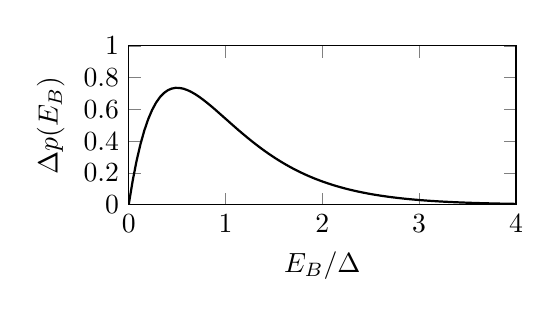
\begin{tikzpicture}\begin{axis}[width=6.5cm,height=3.6cm,xmin=0,xmax=4,ymin=0,ymax=1,xlabel={$E_B/\Delta$},ylabel={$\Delta p(E_B)$}]\addplot[domain=0:4,thick,samples=100]{4*x*exp(-2*x)};\end{axis}\end{tikzpicture}\hspace{.2cm}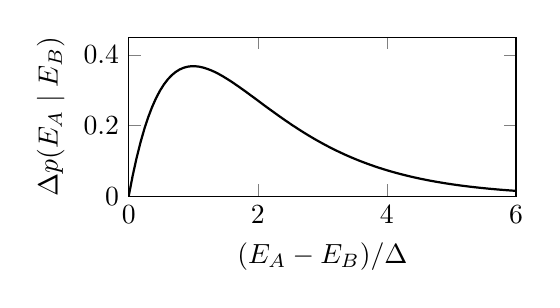
\begin{tikzpicture}\begin{axis}[width=6.5cm,height=3.6cm,xmin=0,xmax=6,ymin=0,ymax=.45,xlabel={$(E_A-E_B)/\Delta$},ylabel={$\Delta p(E_A\mid E_B)$}]\addplot[domain=0:6,thick,samples=100]{x*exp(-x)};\end{axis}\end{tikzpicture}\end{center}
\originalsection{2．表面极性分子（30 分）}
\begin{exercise}
$N$ 个吸附极性分子在垂直电场 $\mathcal E$ 中总电偶极矩 $\mathcal P$，零场仍可非零。已知
\[\left(\frac{\partial\mathcal P}{\partial\mathcal E}\right)_T=N(a+b/T)+3cN\mathcal E^2,\qquad
\left(\frac{\partial T}{\partial\mathcal E}\right)_{\mathcal P}=\frac{aT^2+bT+3cT^2\mathcal E^2}{b\mathcal E-dT^2},\]
且 $\mathcal P(T_0,0)=P_0$，各小写系数常数。求解析状态方程。
\end{exercise}
\begin{solution}
第一式积分得 $\mathcal P=N(a+b/T)\mathcal E+cN\mathcal E^3+g(T)$。恒 $\mathcal P$ 下 $T_{\mathcal E}=-\mathcal P_{\mathcal E}/\mathcal P_T$，与第二式比较得 $g'=Nd$；故 $\mathcal P=P_0+Nd(T-T_0)+N(a+b/T)\mathcal E+cN\mathcal E^3$。两偏导关系需在坐标变换分母非零的区域理解。
\end{solution}
\originalsection{3．定轴分子固体（40 分）}
\begin{exercise}
$N$ 个固定晶格位分子只有绕 $z$ 轴的经典转动，不相互作用；$0\le\theta_i<2\pi$、$l_i\in\mathbb R$，$H=\sum l_i^2/(2I)$。
(a) 微正则能在 $E,E+\Delta$，$\Delta\ll E$，求相空间壳体积并用 Stirling 简化；(b) 据此求 $p(\theta)$ 并解释；(c) $p(l)=\Omega'/\Omega$，求 $\Omega'$，无须化简，说明如何消去 $E$；(d) 求 $E(T,N)$。
\end{exercise}
\begin{solution}
(a) $N$ 维动量球给
\[\Phi_N=(2\pi)^N\frac{(2\pi I E)^{N/2}}{\Gamma(N/2+1)},\quad
\Omega_N\simeq(2\pi)^N\frac{(2\pi I)^{N/2}E^{N/2-1}\Delta}{\Gamma(N/2)}.\]
计熵时除 $h^N$，不除粒子 $N!$，因为位置固定可区分。领先大 $N$ 形式 $\Omega_N\simeq(2\pi)^N(4\pi eIE/N)^{N/2}N\Delta/(2E)$，略去次广延因子。
(b) 所有角可达体积相同，$p(\theta)=1/(2\pi)$。
(c) 固定 $l$、仍积分它的角，$\Omega'=2\pi\Omega_{N-1}(E-l^2/(2I),\Delta)$（采用原始有量纲体积）；支持 $l^2/(2I)<E$。若采用无量纲计数，则比值另乘 $2\pi/h$。代 (d) 可消去 $E$，大 $N$ 得方差 $I\kb T$ 的高斯。
(d) 壳熵精确领先导数为 $E=(N/2-1)\kb T$；原卷大系统舍去 $\ln[N\Delta/(2E)]$ 等次广延项，得到 $E=N\kb T/2$，即均分结果。
\end{solution}
